\documentclass[fleqn]{scrreprt}

\usepackage{graphicx}
\usepackage{rotating}
\usepackage{amsmath}
\usepackage{hyperref}

\graphicspath{ {img/} }

\title{COMP3005 Project Report}
\author{Yannick Abouem - Student\# 101151033}

\begin{document}
\maketitle

\tableofcontents

\chapter{Conceptual Design}
\section{Cardinalities and Participation Types Explanation}
Following is a more detailed overview of each relationship with an explanation
of its cardinality and participation from member entities, as well as a closer
look to the member entities.

\subsection{Has Relationship}
The Has Relationship occurs between the User entity and the Checkout Basket
weak entity and its the identifying relationship for Checkout Basket.
This relationship has a 1:1 cardinality with total participation the Checkout
Basket and partial participation for the User Entity.
The cardinality is such because each User can only have one Checkout
Basket and Checkout Baskets are not shared between users. The relationship
requires total participation for the Checkout Basket entity since its the
identifying relationship for the Checkout Basket and the User's checkout basket
might be created when needed.
\begin{figure}[h]\centering
    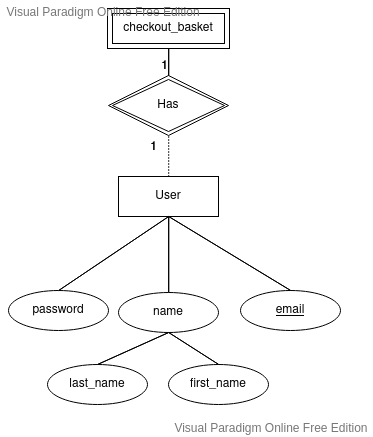
\includegraphics[width=.5\columnwidth]{er-diagram-project-Has.vpd.png}
    \caption{Has relationship ER-diagram}\label{fig:erh}
\end{figure}

\subsection{In Basket Relationship}
The In Basket relationship occurs between the Book entity and the Checkout Basket
weak entity. This relationship is a N:M relationship with partial participation
for both entities. The N:M cardinality is used for this relationship as each
book can be in multiple checkout baskets simultaneously and each checkout basket
can have multiple different books. Both entities have a optional participation
in this relationship as both entities can exists without being in this relationship.
For example a book does not have to be in a basket if its not being purchased
and a checkout basket can be empty and still exist.
\begin{figure}[h]\centering
    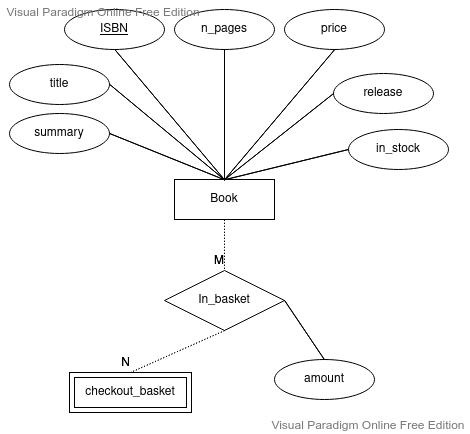
\includegraphics[width=.7\columnwidth]{er-diagram-project-In-Basket.vpd.png}
    \caption{In Basket relationship ER-diagram}\label{fig:erib}
\end{figure}

\subsection{Is Genre}
This relationship occurs between the Genre and Book relationship and its a N:M
relationship with total participation for both entities. The cardinality of
this relationship is N:M because each book can have multiple genre and each
genre has a list of books which belongs to it. While the participation is total
for both entities because books are classified by genre and therefore all books
must have a genre. While genres which do not have at leas a book associated to
it has no reason to be in the database.
\begin{figure}[ht]\centering
    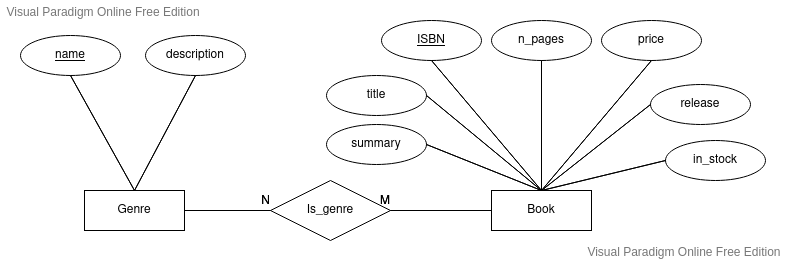
\includegraphics[width=.7\columnwidth]{er-diagram-project-Is-Genre.vpd.png}
    \caption{Is Genre relationship ER-diagram}\label{fig:erig}
\end{figure}

\subsection{Ordered}
The Ordered relationship connects the Book entity and the Order entity with
a N:M cardinality and total participation for the Order entity and partial
participation for the Book entity. The N:M cardinality is due to the fact that
each order can have multiple books and each book can be placed in multiple
different orders. The Order entity's total participation is caused by the nature
of the order itself (i.e. we cannot have empty orders) while the partial participation
for the Book entity is caused by the fact that a book does not have to be ordered
in order to exists in the database. This relationship also has an attribute
called amount. This attribute serves to simplify the ordering of the same
book multiple times.
\begin{figure}[h]\centering
    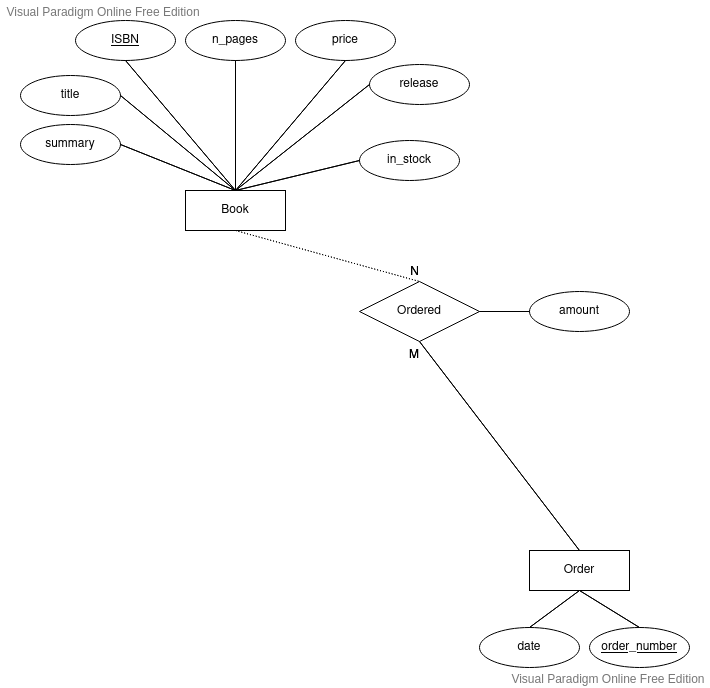
\includegraphics[width=.6\columnwidth]{er-diagram-project-Ordered.vpd.png}
    \caption{Ordered relationship ER-diagram}\label{fig:ero}
\end{figure}

\subsection{Payment}
This relationship connects the Order entity and the Billing Info weak entity
and is the defining relationship of the latter. It's a 1:1 relationship with
total participation for the Billing Info entity and partial for the Order entity.
This is a fairly straight forward
relationship which serves to connect the order to its payment informations. Each
order can only have one payment information and one payment information has
one order since payment informations must not be shared between orders since
there is the potential risk of leaking the user banking informations. Similarly
the relationship requires total participation for the Billing Info since these
informations are part of the order. While its a partial 
\begin{figure}[h]\centering
    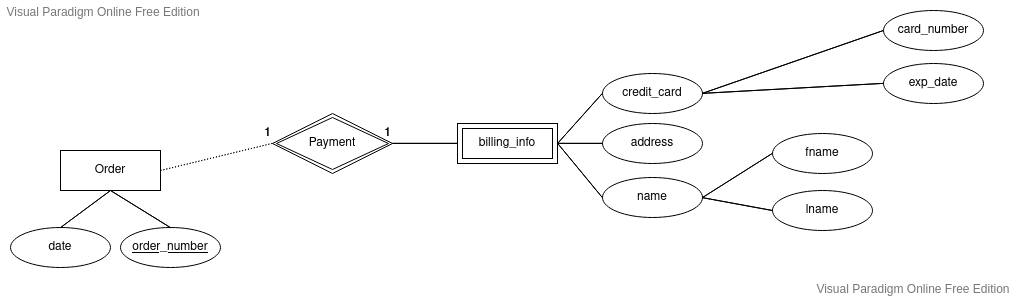
\includegraphics[width=\columnwidth]{er-diagram-project-Payment.vpd.png}
    \caption{Payment relationship ER-diagram}\label{fig:erp}
\end{figure}

\subsection{Places}
This 1:N relationship occurs between the User entity and the Order entity. It
has a partial participation for the User and a total participation for the Order.
Each user can create and own N orders while each order can have only one user,
orders cannot be shared or owned by multiple users. Users do not have to place
an order, hence the partial participation, while orders must have a user who
owns said order.
\begin{figure}[h]\centering
    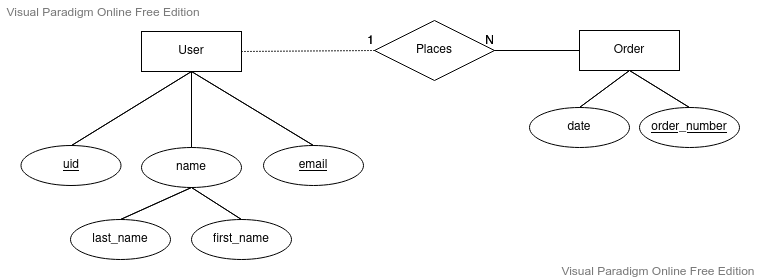
\includegraphics[width=.8\columnwidth]{er-diagram-project-Places.vpd.png}
    \caption{Places relationship ER-diagram}\label{fig:erpl}
\end{figure}

\subsection{Publish}
This 1:N relationship occurs between the Book entity and the Publisher entity.
This relationship is due to the fact that each Book only has one publisher and
each publisher can publish multiple books. Both entities have a total
participation as books have to be published and publishers without published
books are of no use in this application. This relationship has an attribute
Publisher Percentage which serves to indicate how much the publisher will gain
from the sale of the specified book.
\begin{figure}[h]\centering
    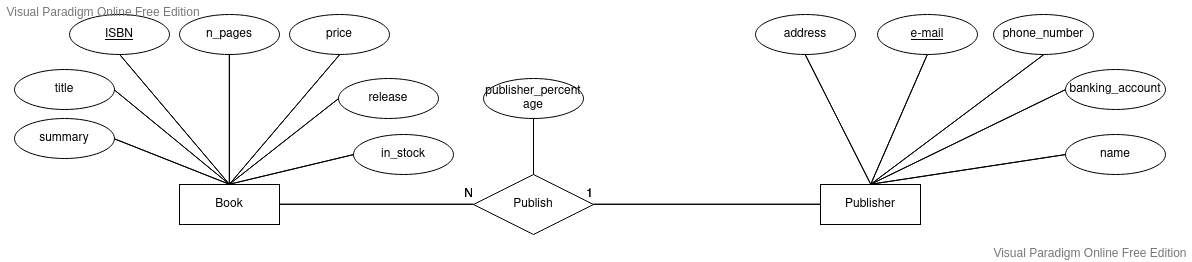
\includegraphics[width=\columnwidth]{er-diagram-project-Publish.vpd.png}
    \caption{Publish relationship ER-diagram}\label{fig:erpu}
\end{figure}

\newpage
\subsection{Ship To}
The Ship To relationship is a 1:1 relationship which requires total participation
from the Shipping Info weak entity, since it's its defining relationship,
and partial participation from the Order entity. This is due to the fact
that each order only has one address that needs to be delivered to and shipping
informations are not shared between orders. The partial participation with the
Order entity is due to redundancy since its possible to use billing informations
as shipping informations.
\begin{figure}[h]\centering
    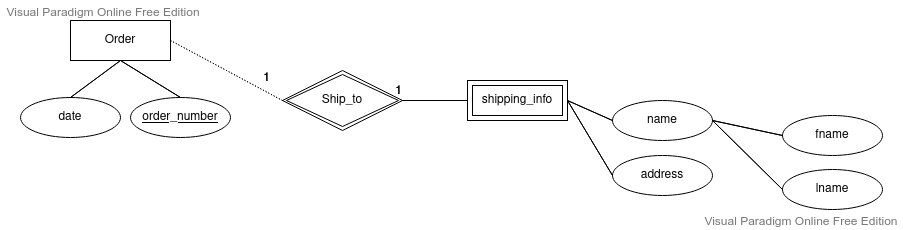
\includegraphics[width=\columnwidth]{er-diagram-project-Ship-To.vpd.png}
    \caption{Ship To relationship ER-diagram}\label{fig:erst}
\end{figure}

\subsection{Tracks}
This 1:1 relationship is the defining relationship of the Tracking Information
entity and connects it to the Order entity. Total participation is required for
the Tracking Information entity since each tracking information cannot exist on
is own and partial for the Order entity since orders which are not shipped yet
have not shipping information. Each order only has one tracking information.
\begin{figure}[h]\centering
    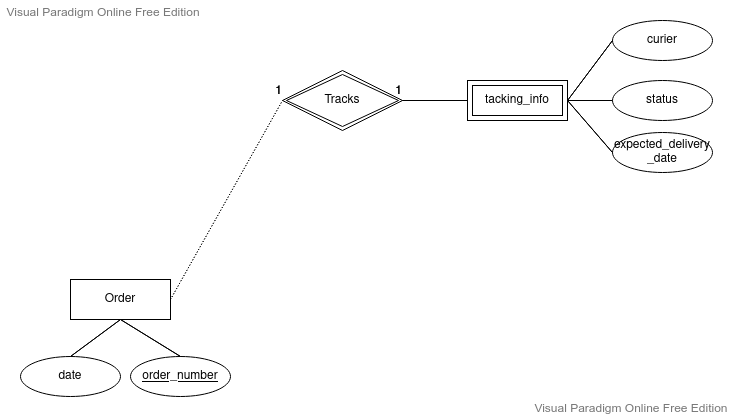
\includegraphics[width=.8\columnwidth]{er-diagram-project-Tracks.vpd.png}
    \caption{Tracks relationship ER-diagram}\label{fig:ert}
\end{figure}

\subsection{Wrote}
The Wrote relationship occurs between the Author and Book entities. Its a N:M
relationship with total participation required for both entities. This is due to
the fact that each author can write multiple books and some books are co-authored
by multiple authors. There are no books that don't have a author (books with
unknown author can be created with an author named unknown) and authors without
books are irrelevant for our application.
\begin{figure}[ht]\centering
    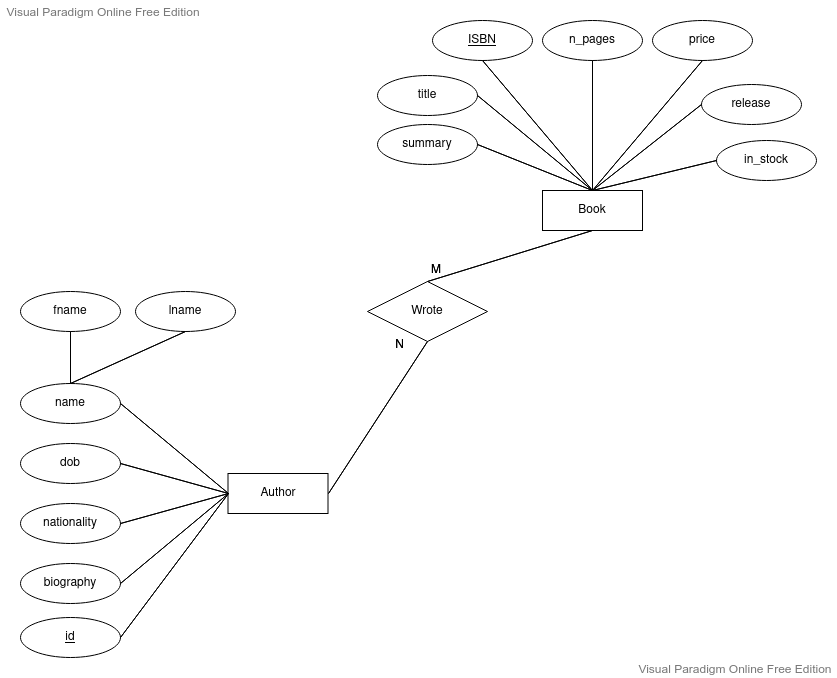
\includegraphics[width=.8\columnwidth]{er-diagram-project-Wrote.vpd.png}
    \caption{Wrote relationship ER-diagram}\label{fig:erw}
\end{figure}
\newpage
\section{Full ER-Diagram}
In the following page you can find the full ER-Diagram for the database.
\begin{sidewaysfigure}[ht]\centering
    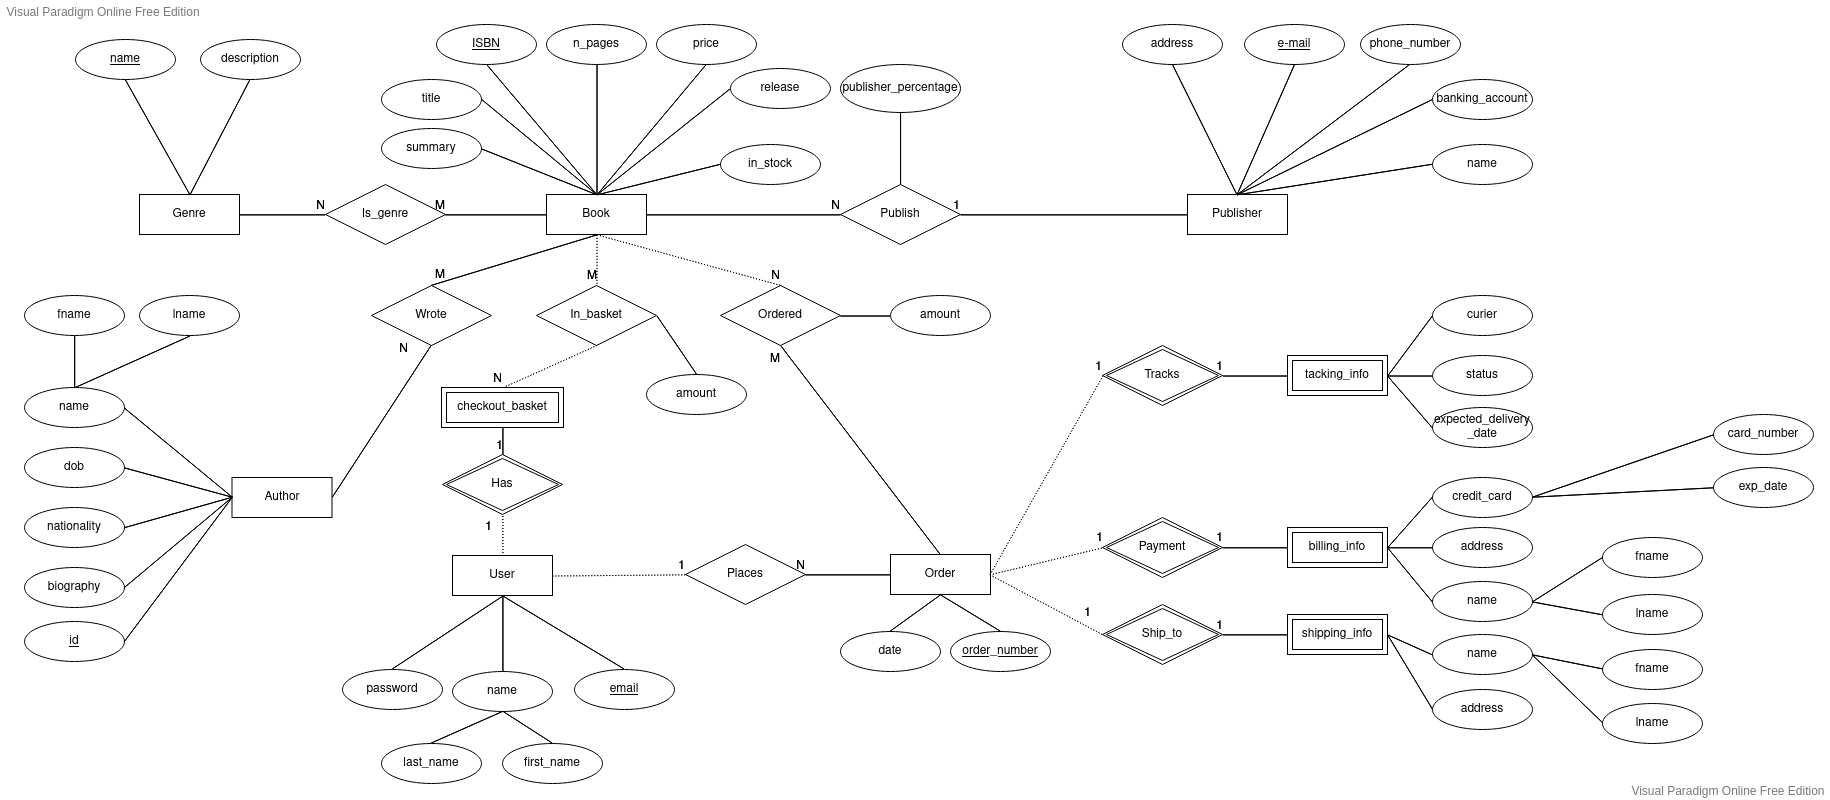
\includegraphics[width=\columnwidth]{er-diagram-project.vpd.png}
    \label{fig:erfull}
\end{sidewaysfigure}

\chapter{Relation Schemas}
\section{Relation Schemas Reduced From ER-Diagram}
Following is the list of relation schemas reduced from the ER-Diagram.
\begin{figure}[h]\centering
    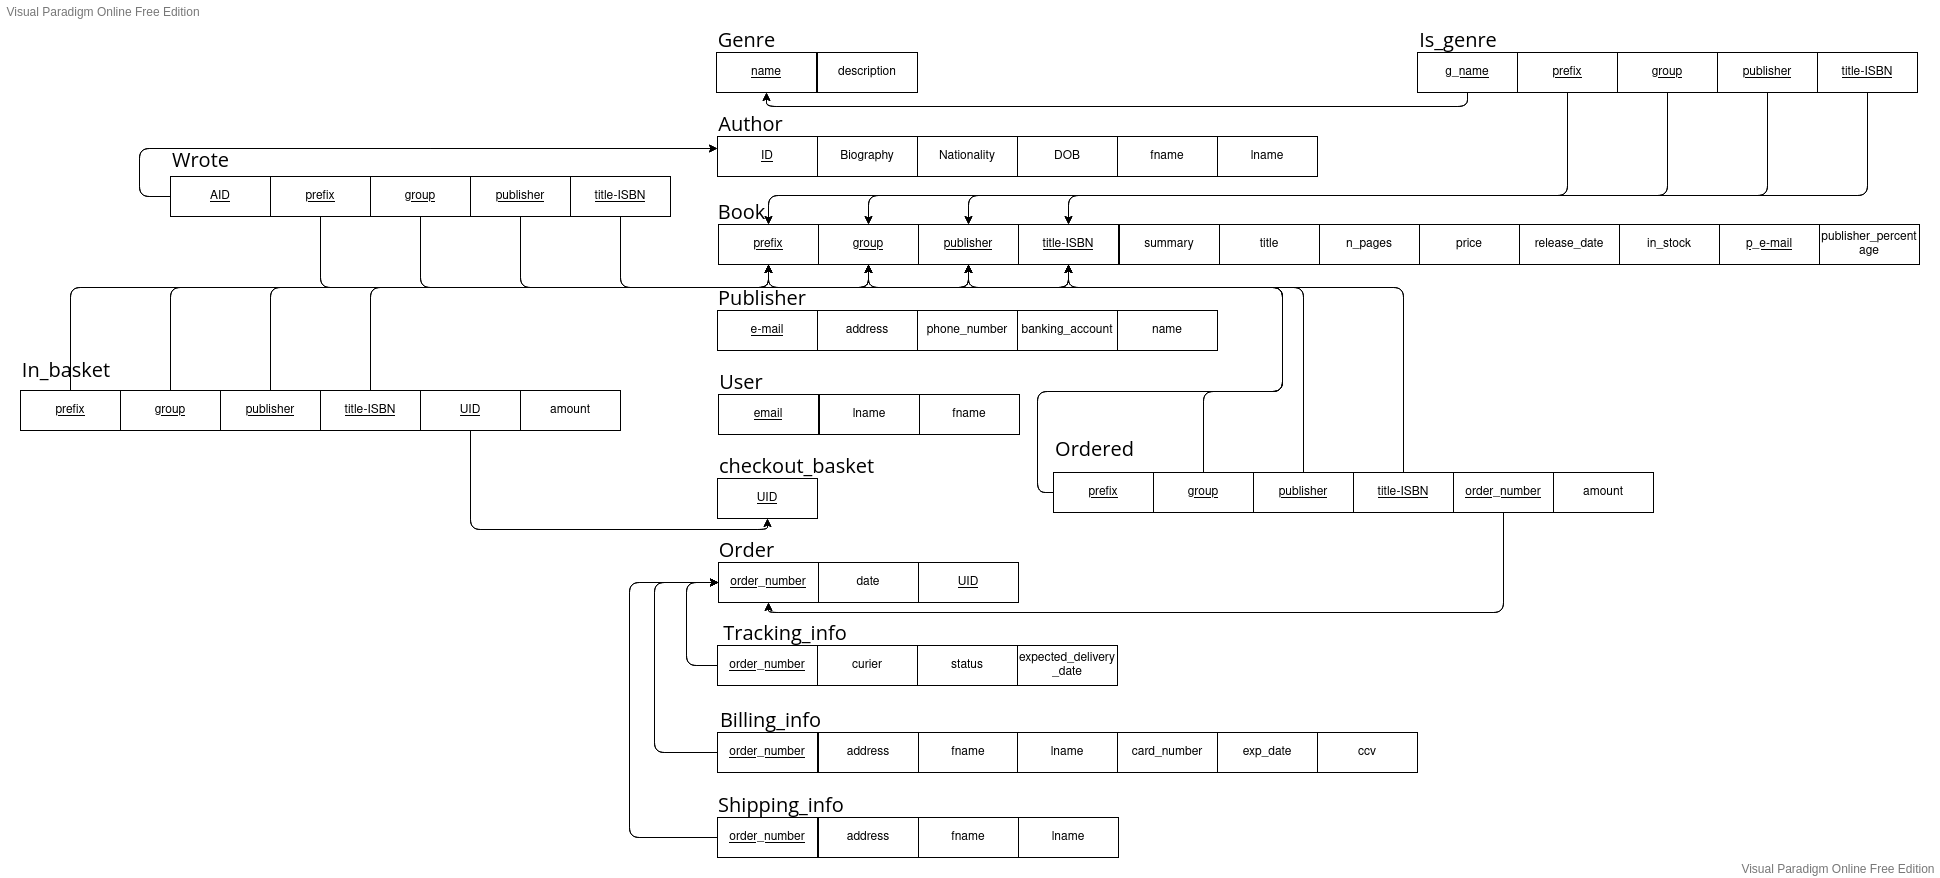
\includegraphics[width=\columnwidth]{relational-schema.vpd.png}
    \label{fig:rs}
\end{figure}

\newpage
\section{Normalization of Relation Schemas}
\subsection{Normal Form Test}
\subsubsection{Genre}
\begin{equation*}
    R = genre(name, description)
\end{equation*}
\begin{equation*}
    F = \{name \rightarrow description\}
\end{equation*}
Calculate $(name)^+$
\begin{align*}
    & result = name\\
    & name \rightarrow description : result = name, description\\
    & (name)^+ = name, description\\
    & (name)^+ = R
\end{align*}
Genre is in BCNF.

\subsubsection{Author}
\begin{equation*}
    R = author(ID, bio, nationality, DOB, fname, lname)
\end{equation*}
\begin{align*}
    F = \{ & ID \rightarrow bio\\
          & ID \rightarrow nationality\\
          & ID \rightarrow DOB\\
          & ID \rightarrow fname, lname \}
\end{align*}
Calculate if $ID$ is a superkey of $R$
\begin{align*}
    & (ID)^+\\
    & result = ID\\
    & ID \rightarrow bio : result = ID, bio\\
    & ID \rightarrow nationality : result = ID, bio, nationality\\
    & ID \rightarrow DOB : result = ID, bio, nationality, DOB\\
    & ID \rightarrow fname, lname : result = ID, bio, nationality, DOB, fname, lname\\
    & (ID)^+ = ID, bio, nationality, DOB, fname, lname
\end{align*}
Therefore $ID$ is superkey of $author$ and the relational schema is in BCNF.

\newpage
\subsubsection{Book}
\begin{multline*}
    R = book(prefix, group, ISBN, summary, title, n\_pages,\\
    price, release\_date, in\_stock, p\_email, publisher\_percentage)
\end{multline*}
\begin{align*}
    F = \{ & ISBN \rightarrow summary\\
          & ISBN \rightarrow title\\
          & ISBN \rightarrow n\_pages\\
          & ISBN \rightarrow price\\
          & ISBN \rightarrow release\_date\\
          & ISBN \rightarrow in\_stock\\
          & publisher \rightarrow p\_email\\
          & ISBN \rightarrow publisher\_precentage\}
\end{align*}

Calculate if $ISBN$ is superkey of $R$
\begin{align*}
    & (ISBN)^+\\
    & result = ISBN\\
    & ISBN \rightarrow summary : result = ISBN, summary\\
    & ISBN \rightarrow title : result = ISBN, summary, title\\
    & ISBN \rightarrow n\_pages : result = ISBN, summary, title, n\_pages\\
    & ISBN \rightarrow price : result = ISBN, summary, title, n\_pages, price\\
    & ISBN \rightarrow release\_date : result = ISBN, summary, title, n\_pages\\
    & price, release\_date\\
    & ISBN \rightarrow in\_stock : result = ISBN, summary, title, n\_pages\\
    & prices, release\_date, in\_stock\\
    & ISBN \rightarrow p\_email : result = ISBN, summary, title, n\_pages\\
    & prices, release\_date, in\_stock, p\_email\\
    & ISBN \rightarrow publisher\_precentage\ : result = ISBN, summary, title\\
    & n\_pages, prices, release\_date, in\_stock, p\_email, publisher\_percentage\\
    & (ISBN)^+ = ISBN, summary, title, n\_pages, prices, release\_date,\\
    & in\_stock, p\_email, publisher\_percentage\\
\end{align*}
Therefore $ISBN$ is superkey of $Book$ and the relational schema is in BCNF.

\newpage
\subsubsection{Publisher}
\begin{equation*}
    R = publisher(e\-mail, address, phone\_number, banking\_account, name)
\end{equation*}
\begin{align*}
    F = \{ & e\-mail \rightarrow address\\
           & e\-mail \rightarrow phone\_number\\
           & e\-mail \rightarrow banking\_account\\
           & e\-mail \rightarrow name\}
\end{align*}

Find if $email$ is superkey of $R$:
\begin{align*}
    & (email)^+\\
    & result = email\\
    & e\-mail \rightarrow address : result = email, address\\
    & e\-mail \rightarrow phone\_number : result = email, address, phone\_number\\
    & e\-mail \rightarrow banking\_account : result = email, address\\
    & phone\_number, banking\_account\\
    & e\-mail \rightarrow name : result = email, address, phone\_number\\
    & banking\_account, name\\
    & (email)^+ = email, address, phone\_number, banking\_account, name\\
\end{align*}

Since $email$ is superkey of $R$ no relation causes a violation of BCNF,
therefore Publisher is in normal form.

\subsubsection{User}
\begin{equation*}
    R = user{email, lname, fname, password}
\end{equation*}
\begin{align*}
    F = \{ & emali \rightarrow lname\\
           & email \rightarrow fname\\
           & email \rightarrow password\}
\end{align*}

Normal form test of $R$ by finding if $email$ is superkey.
\begin{align*}
    & (email)^+\\
    & result = email\\
    & emali \rightarrow lname : result = email, lname\\
    & emali \rightarrow fname : result = email, lname, fname\\
    & emali \rightarrow password : result = email, lname, fname, password\\
    & (email)^+ = email, lanme, fname, password\\
    & (email)^+ = R
\end{align*}
$email$ is superkey of $R$, therefore no functional dependency in $F$ is in
violation of BCNF and user is in normal form.

\subsubsection{Checkout Basket}
\begin{equation*}
    R = checkout_basket(email)
\end{equation*}
\begin{equation*}
    F = \{email \rightarrow email\}
\end{equation*}

The functional dependency $email \rightarrow email$ is trivial and the only
functional relation. Therefore checkout basket is in normal form.

\subsubsection{Order}
\begin{equation*}
    R = order(order\_number, date, email)
\end{equation*}
\begin{equation*}
    F = \{ order\_number \rightarrow date, email \}
\end{equation*}

Normal form test for $R$ by finding if $order\_number$ is superkey.
\begin{align*}
    & (order\_numner)^+\\
    & result = order\_number\\
    & order\_number \rightarrow date, email : result = order\_number, date, email\\
    & (order\_number)^+ = order\_number, date, email\\
    & (order\_number)^+ = R
\end{align*}

Since $order\_number$ superkey of $R$ and no functional dependency is in violation
of BCNF, then order is in normal form.

\subsubsection{Tracking Info}
\begin{equation*}
    R = tracking\_info(order\_number, curier, status, expected\_delivery\_date)
\end{equation*}
\begin{align*}
    F = \{ & oredr\_number \rightarrow curier\\
           & order\_number \rightarrow status\\
           & order\_number \rightarrow expected\_delivery\_date \}
\end{align*}

Normal form test for $R$ by finding if $order\_number$ is superkey.
\begin{align*}
    & (order\_number)^+\\
    & result = order\_number\\
    & oredr\_number \rightarrow curier : result = order\_number, curier\\
    & oredr\_number \rightarrow status : result = order\_number, curier, status\\
    & oredr\_number \rightarrow expected\_delivery\_date : result = order\_number\\
    & curier, status, expected\_delivery\_date\\
    & (order\_number)^+ = order\_number, curier, status, expected\_delivery\_date\\
    & (order\_number)^+ = R
\end{align*}

Since $order\_number$ superkey of $R$ and no functional dependency is in violation
of BCNF, then tracking info is in normal form.

\subsubsection{Billing Info}
\begin{equation*}
    R = billing\_info(order\_number, address, fname, lname, card\_number, exp\_date)
\end{equation*}
\begin{align*}
    F = \{ & order\_number \rightarrow address\\
           & order\_number \rightarrow fname, lname\\
           & order\_number \rightarrow card\_number\\
           & order\_number \rightarrow exp\_date \}
\end{align*}

Normal form test for $R$ by finding if $order\_number$ is superkey.
\begin{align*}
    & (order\_number)^+\\
    & result = order\_number\\
    & order\_number \rightarrow address : result = order\_number, address\\
    & order\_number \rightarrow fname, lname : result = order\_number, address,\\
    & fname, lname\\
    & order\_number \rightarrow card\_number : result = order\_number, address,\\
    & fname, lname, card\_number\\
    & order\_number \rightarrow exp\_date : result = order\_number, address,\\
    & fname, lname, card\_number, exp\_date\\
    & (order\_number)^+ = order\_number, address, fname, lname, card\_number,\\
    & exp\_date\\
    & (order\_number)^+ = R
\end{align*}

Since $order\_number$ superkey of $R$ and no functional dependency is in violation
of BCNF, then billing info is in normal form.

\subsubsection{Shipping Info}
\begin{equation*}
    R = shipping\_info(order\_number, address, fname, lname)
\end{equation*}
\begin{align*}
    F = \{ & order\_number \rightarrow address\\
           & order\_number \rightarrow fname, lname \}
\end{align*}

Normal form test for $R$ by finding if $order\_number$ is superkey.
\begin{align*}
    & (order\_number)^+\\
    & result = order\_number\\
    & order\_number \rightarrow address : result = order\_number, address\\
    & order\_number \rightarrow fname, lname : result = order\_number, address,\\
    & fname, lname\\
    & (order\_number)^+ = order\_number, address, fname, lname\\
    & (order\_number)^+ = R
\end{align*}

Since $order\_number$ superkey of $R$ and no functional dependency is in violation
of BCNF, then shipping info is in normal form.

\chapter{Database Schema Diagram}
Here you can find the final schema diagram of the database.
\begin{figure}[h]\centering
    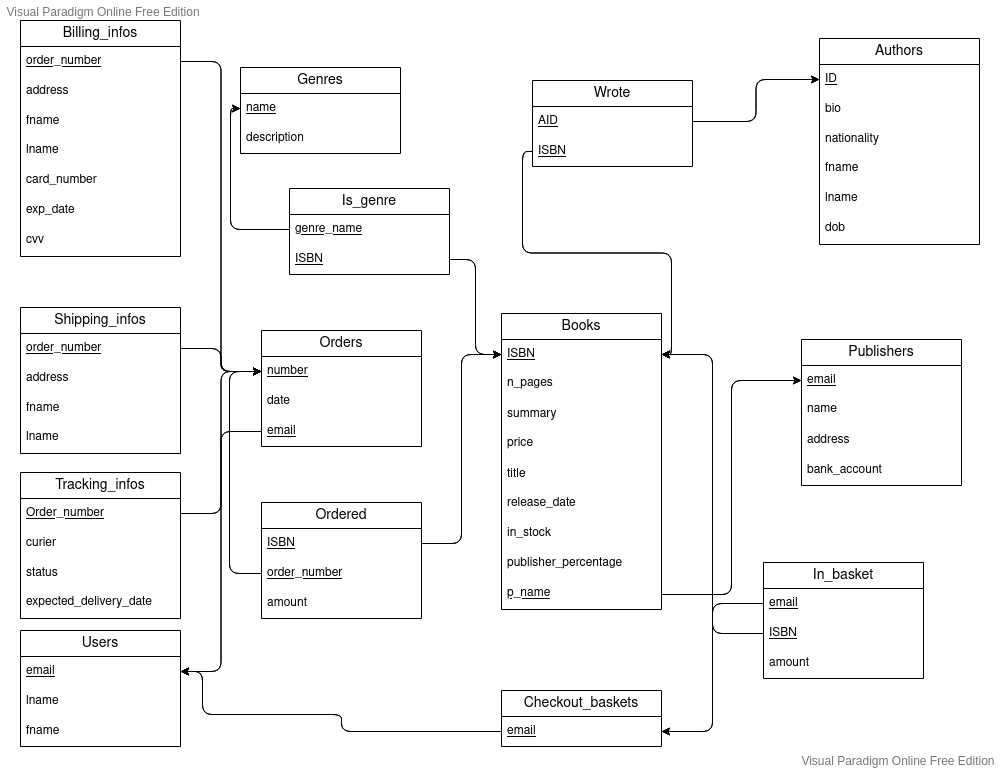
\includegraphics[width=\columnwidth]{database-schema-diagram.vpd.png}
    \label{fig:dsd}
\end{figure}

\chapter{Implementation}
\section{Architecture}
The implementation of the book store is a web based application developed using
Integrated Haskell Platform (IHP) and the Haskell programming language. The
application follows the MVC (Model-View-Controller) structure. It has an application
called Web which deals with the front end of the website. Here requests will be
processed by the Controllers which will respond to the request with a View.

Most of the routing work is handled by the Book controller located in the Web/Controller/Books.hs
file. Here different requests are routed requesting different informations from
the database. This file is supposed to deal with simple queries as well but
more complex queries and queries which require a JOIN operation are located
in the Application/BooksQuery.hs file. This is due to how IHP and Haskell work
with types, writing complex queries which will return new tables not defined
in the schema will require a new custom data type. You can find these datatypes
in the same file.

\section{GitHub Repository}
\url{https://github.com/AntaresMKII/COMP3005-project}

\chapter{Appendix}
Availability:
\begin{itemize}
    \item 10am
    \item 11am
    \item 1pm
\end{itemize}
\end{document}
